\noindent{\small\textbf{CIÊNCIAS DA NATUREZA E SUAS TECNOLOGIAS}}

\noindent\textbf{Questões \ref{cn-first} a \ref{cn-last}} %arrumar o número

%
% Biologia - Luan
%

\questao \label{cn-first}
Nas recentes expedições espaciais que chegaram ao solo de Marte, e através dos sinais fornecidos por diferentes sondas e formas de análise, vem sendo investigada a possibilidade da existência de água naquele planeta. A motivação principal dessas investigações, que ocupam frequentemente o noticiário sobre Marte, deve-se ao fato de que a presença de água indicaria, naquele planeta:
\begin{alternativas}
\item a existência de um solo rico em nutrientes e com potencial para a agricultura. 
\item a existência de ventos, com possibilidade de erosão e formação de canais. 
\item a possibilidade de existir ou ter existido alguma forma de vida semelhante à da Terra. 
\item a possibilidade de extração de água visando ao seu aproveitamento futuro na Terra. 
\item a viabilidade, em futuro próximo, do estabelecimento de colônias humanas em Marte.
\end{alternativas}

\questao
\citacao{
Um molusco, que vive no litoral oeste dos EUA, pode redefinir tudo o que se sabe sobre a divisão entre animais e vegetais. Isso porque o molusco (\textit{Elysia chlorotica}) é um híbrido de bicho com planta. Cientistas americanos descobriram que o molusco conseguiu incorporar um gene das algas e, por isso, desenvolveu a capacidade de fazer fotossíntese. É o primeiro animal a se “alimentar” apenas de luz e CO2, como as plantas.}{
GARATONI, B. Superinteressante. Edição 276, mar. 2010 (adaptado).}
A capacidade de o molusco fazer fotossíntese deve estar associada ao fato de o gene incorporado permitir que ele passe a sintetizar:
\begin{alternativas}
\item clorofila, que utiliza a energia do carbono para produzir glicose. 
\item citocromo, que utiliza a energia da água para formar oxigênio. 
\item clorofila, que doa elétrons para converter gás carbônico em oxigênio. 
\item citocromo, que doa elétrons da energia luminosa para produzir glicose. 
\item clorofila, que transfere a energia da luz para compostos orgânicos.
\end{alternativas}

\questao
Em certos locais, larvas de moscas, criadas em arroz cozido, são utilizadas como iscas para pesca. Alguns criadores, no entanto, acreditam que essas larvas surgem espontaneamente do arroz cozido, tal como preconizado pela teoria da geração espontânea. Essa teoria começou a ser refutada pelos cientistas ainda no século XVII, a partir dos estudos de Redi e Pasteur, que mostraram experimentalmente que:
\begin{alternativas}
\item seres vivos podem ser criados em laboratório. 
\item a vida se originou no planeta a partir de microrganismos. 
\item o ser vivo é oriundo da reprodução de outro ser vivo preexistente. 
\item seres vermiformes e microrganismos são evolutivamente aparentados. 
\item vermes e microrganismos são gerados pela matéria existente nos cadáveres e nos caldos nutritivos, respectivamente.
\end{alternativas}

\questao
O gráfico abaixo representa a evolução da quantidade de oxigênio na atmosfera no curso dos tempos geológicos. O número 100 sugere a quantidade atual de oxigênio na atmosfera, e os demais valores indicam diferentes porcentagens dessa quantidade.
\begin{center}
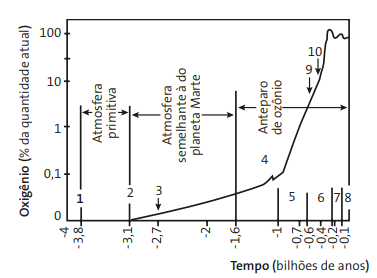
\includegraphics[width=\columnwidth]{subareas/ciencias_natureza/biologia-1.png}
\end{center}
De acordo com o gráfico é correto afirmar que:
\begin{alternativas}
\item as primeiras formas de vida surgiram na ausência de O2. 
\item a atmosfera primitiva apresentava 1\% de teor de oxigênio. 
\item após o início da fotossíntese, o teor de oxigênio na atmosfera mantém-se estável. 
\item desde o Pré-Cambriano, a atmosfera mantém os mesmos níveis de teor de oxigênio. 
\item na escala evolutiva da vida, quando surgiram os anfíbios, o teor de oxigênio atmosférico já se havia estabilizado.
\end{alternativas}

\questao
A partir do primeiro semestre de 2000, a ocorrência de casos humanos de febre amarela silvestre extrapolou as áreas endêmicas, com registro de casos em São Paulo e na Bahia, onde os últimos casos tinham ocorrido em 1953 e 1948. Para controlar a febre amarela silvestre e prevenir o risco de uma reurbanização da doença, foram propostas as seguintes ações: \\
I. Exterminar os animais que servem de reservatório do vírus causador da doença. \\
II. Combater a proliferação do mosquito transmissor. \\
III. Intensificar a vacinação nas áreas onde a febre é endêmica e em suas regiões limítrofes.\\
É efetiva e possível de ser implementada uma estratégia envolvendo a(s) ação(ões): 
\begin{alternativas}
\item II, apenas. 
\item I e II, apenas. 
\item I e III, apenas.
\item II e III, apenas. 
\item I, II e III.
\end{alternativas}

\questao
Na embalagem de um antibiótico, encontra-se uma bula que, entre outras informações, explica a ação do remédio do seguinte modo: ``O medicamento atua por inibição da síntese proteica bacteriana''. Essa afirmação permite concluir que o antibiótico: 
\begin{alternativas}
\item impede a fotossíntese realizada pelas bactérias causadoras da doença e, assim, elas não se alimentam e morrem. 
\item altera as informações genéticas das bactérias causadoras da doença, o que impede a manutenção e a reprodução desses organismos. 
\item dissolve as membranas das bactérias responsáveis pela doença, o que dificulta o transporte de nutrientes e provoca a morte delas.
\item elimina os vírus causadores da doença, pois não conseguem obter as proteínas que seriam produzidas pelas bactérias que parasitam. 
\item interrompe a produção de proteína das bactérias causadoras da doença, o que impede sua multiplicação pelo bloqueio de funções vitais.
\end{alternativas}

\questao
O que têm em comum Noel Rosa, Castro Alves, Franz Kafka, Álvares de Azevedo, José de Alencar e Frédéric Chopin? Todos eles morreram de tuberculose, doença que ao longo dos séculos fez mais de 100 milhões de vítimas. Aparentemente controlada durante algumas décadas, a tuberculose voltou a matar. O principal obstáculo para seu controle é o aumento do número de linhagens de bactérias resistentes aos antibióticos usados para combatê-la. Esse aumento do número de linhagens resistentes se deve a: 
\begin{alternativas}
\item modificações no metabolismo das bactérias, para neutralizar o efeito dos antibióticos e incorporá-los à sua nutrição. 
\item mutações selecionadas pelos antibióticos, que eliminam as bactérias sensíveis a eles, mas permitem que as resistentes se multipliquem. 
\item mutações causadas pelos antibióticos, para que as bactérias se adaptem e transmitam essa adaptação a seus descendentes. 
\item modificações fisiológicas nas bactérias, para torná-las cada vez mais fortes e mais agressivas no desenvolvimento da doença. 
\item modificações na sensibilidade das bactérias, ocorridas depois de passarem um longo tempo sem contato com antibióticos.
\end{alternativas}

\questao
Os anfíbios são animais que apresentam dependência de um ambiente úmido ou aquático. Nos anfíbios, a pele é de fundamental importância para a maioria das atividades vitais, apresenta glândulas de muco para conservar-se úmida, favorecendo as trocas gasosas e, também, pode apresentar glândulas de veneno contra microrganismos e predadores. Segundo a Teoria Evolutiva de Darwin, essas características dos anfíbios representam a:
\begin{alternativas}
\item lei do uso e desuso. 
\item atrofia do pulmão devido ao uso contínuo da pele. 
\item transmissão de caracteres adquiridos aos descendentes. 
\item futura extinção desses organismos, pois estão mal adaptados. 
\item seleção de adaptações em função do meio ambiente em que vivem.
\end{alternativas}

\questao
Fenômenos biológicos podem ocorrer em diferentes escalas de tempo. Assinale a opção que ordena exemplos de fenômenos biológicos, do mais lento para o mais rápido.
\begin{alternativas}
\item germinação de uma semente, crescimento de uma árvore, fossilização de uma samambaia 
\item fossilização de uma samambaia, crescimento de uma árvore, germinação de uma semente 
\item crescimento de uma árvore, germinação de uma semente, fossilização de uma samambaia 
\item fossilização de uma samambaia, germinação de uma semente, crescimento de uma árvore
\item germinação de uma semente, fossilização de uma samambaia, crescimento de uma árvore
\end{alternativas}

\questao
\citacao{
O menor tamanduá do mundo é solitário e tem hábitos noturnos, passa o dia repousando, geralmente em um emaranhado de cipós, com o corpo curvado de tal maneira que forma uma bola. Quando em atividade, se locomove vagarosamente e emite som semelhante a um assobio. A cada gestação, gera um único filhote. A cria é deixada em uma árvore à noite e é amamentada pela mãe até que tenha idade para procurar alimento. As fêmeas adultas têm territórios grandes e o território de um macho inclui o de várias fêmeas, o que significa que ele tem sempre diversas pretendentes à disposição para namorar!}{
Ciência Hoje das Crianças, ano 19, n. 174, nov. 2006 (adaptado).}
Essa descrição sobre o tamanduá diz respeito ao seu:
\begin{alternativas}
\item habitat. 
\item biótopo. 
\item nível trópico. 
\item nicho ecológico. 
\item potencial biótico.
\end{alternativas}

%
% Química - Luan
%

\questao %Enem - MEC
O sol participa do ciclo da água, pois, além de aquecer a superfície da Terra dando origem aos ventos, provoca a evaporação da água dos rios, lagos e mares. O vapor da água, ao se resfriar, condensa em minúsculas gotinhas, que se agrupam formando as nuvens, neblinas ou névoas úmidas. As nuvens podem ser levadas pelos ventos de uma região para outra. Com a condensação e, em seguida, a chuva, a água volta à superfície da Terra, caindo sobre o solo, rios, lagos e mares. Parte dessa água evapora retornando à atmosfera, outra parte escoa superficialmente ou infiltra-se no solo, indo alimentar rios e lagos. Esse processo é chamado de ciclo da água.\\
Considere, então, as seguintes afirmativas:\\
I. A evaporação é maior nos continentes, uma vez que o aquecimento ali é maior do que nos oceanos.\\
II. A vegetação participa do ciclo hidrológico por meio da transpiração.\\
III. O ciclo hidrológico condiciona processos que ocorrem na litosfera, na atmosfera e na biosfera.\\
IV. A energia gravitacional movimenta a água dentro do seu ciclo.\\
V. O ciclo hidrológico é passível de sofrer interferência humana, podendo apresentar desequilíbrios.\\
\begin{alternativas}
\item Somente a afirmativa III está correta.
\item Somente as afirmativas III e IV estão corretas.
\item Somente as afirmativas I, II e V estão corretas.
\item Somente as afirmativas II, III, IV e V estão corretas.
\item Todas as afirmativas estão corretas.
\end{alternativas}

\questao
\citacao{
Quando definem moléculas, os livros geralmente apresentam conceitos como: ``a menor parte da substância capaz de guardar suas propriedades''. A partir de definições desse tipo, a ideia transmitida ao estudante é a de que o constituinte isolado (moléculas) contém os atributos do todo. É como dizer que uma molécula de água possui densidade, pressão de vapor, tensão superficial, ponto de fusão, ponto de ebulição etc. Tais propriedades pertencem ao conjunto, isto é, manifestam-se nas relações que as moléculas mantêm entre si.}{
Adaptado de OLIVEIRA, R. J. ``O mito da substância''. Química Nova na Escola, n. 1, 1995.}
O texto evidencia a chamada visão substancialista que ainda se encontra presente no ensino da Química. Abaixo estão relacionadas algumas afirmativas pertinentes ao assunto.\\
I. O ouro é dourado, pois seus átomos são dourados.\\
II. Uma substância “macia” não pode ser feita de moléculas “rígidas”.\\
III. Uma substância pura possui pontos de ebulição e fusão constantes, em virtude dasinterações entre suas moléculas.\\
IV. A expansão dos objetos com a temperatura ocorre porque os átomos se expandem.\\
Dessas afirmativas, estão apoiadas na visão substancialista criticada pelo autor apenas:\\
\begin{alternativas}
\item I e II
\item III e IV
\item I, II e III
\item I, II e IV
\item II, III e IV
\end{alternativas}

\questao
A falta de água doce no planeta será, possivelmente, um dos mais graves problemas deste século. Prevê-se que, nos próximos vinte anos, a quantidade de água doce disponível para cada habitante será drasticamente reduzida. Por meio de seus diferentes usos e consumos, as atividades humanas interferem no ciclo da água, alterando:
\begin{alternativas}
\item a quantidade total, mas não a qualidade da água disponível no planeta.
\item a qualidade da água e sua quantidade disponível para o consumo das populações.
\item a qualidade da água disponível, apenas no subsolo terrestre.
\item apenas a disponibilidade de água superficial existente nos rios e lagos.
\item o regime de chuvas, mas não a quantidade de água disponível no planeta.
\end{alternativas}

\questao
Considerando os custos e a importância da preservação dos recursos hídricos, uma indústria decidiu purificar parte da água que consome para reutilizá-la no processo industrial. De uma perspectiva econômica e ambiental, a iniciativa é importante porque esse processo:
\begin{alternativas}
\item permite que toda água seja devolvida limpa aos mananciais.
\item diminui a quantidade de água adquirida e comprometida pelo uso industrial.
\item reduz o prejuízo ambiental, aumentando o consumo de água.
\item torna menor a evaporação da água e mantém o ciclo hidrológico inalterado.
\item recupera o rio onde são lançadas as águas utilizadas.
\end{alternativas}

\noindent
\textcolor{qgray}{\leaders\vrule height 8pt depth -0.1pt \hfill \null}
\par
\nopagebreak
\vspace{-8pt}
\noindent\rule[3pt]{\columnwidth}{1pt}

\noindent O enunciado abaixo será usado nas questões \textbf{\ref{prodlimp1}} e \textbf{\ref{prodlimp2}}, a seguir:

Produtos de limpeza, indevidamente guardados ou manipulados, estão entre as principais causas de acidentes domésticos. Leia o relato de uma pessoa que perdeu o olfato por ter misturado água sanitária, amoníaco e sabão em pó para limpar um banheiro:

\textbf{``A mistura ferveu e começou a sair uma fumaça asfixiante.''} Não conseguia respirar e meus olhos, nariz e garganta começaram a arder de maneira insuportável. Saí correndo a procura de uma janela aberta para poder voltar a respirar.

\medskip
\questao\label{prodlimp1}
O trecho destacado poderia ser reescrito, em linguagem científica, da seguinte forma:
\begin{alternativas}
\item As substâncias químicas presentes nos produtos de limpeza evaporaram.
\item Com a mistura química, houve produção de uma solução aquosa asfixiante.
\item As substâncias sofreram transformações pelo contato com o oxigênio do ar.
\item Com a mistura, houve transformação química que produziu rapidamente gases tóxicos.
\item Com a mistura, houve transformação química, evidenciada pela dissolução de um sólido.
\end{alternativas}

\questao\label{prodlimp2}
Entre os procedimentos recomendados para reduzir acidentes com produtos de limpeza, aquele que deixou de ser cumprido, na situação discutida na questão anterior, foi:
\begin{alternativas}
\item Não armazene produtos em embalagens de natureza e finalidade diferentes das originais.
\item Leia atentamente os rótulos e evite fazer misturas cujos resultados sejam desconhecidos.
\item Não armazene produtos de limpeza e substâncias químicas em locais próximos a alimentos.
\item Verifique, nos rótulos das embalagens originais, todas as instruções para os primeiros socorros.
\item Mantenha os produtos de limpeza em locais absolutamente seguros, fora do alcance das crianças.
\end{alternativas}

\questao %FUVEST - SP
Thomson determinou, pela primeira vez, a relação entre a massa e a carga do elétron, o que pode ser considerado como a descoberta do elétron. É reconhecida como uma contribuição de Thomson ao modelo atômico,
\begin{alternativas}
\item o átomo ser indivisível.
\item a existência de partículas subatômicas.
\item os elétrons ocuparem níveis discretos de energia.
\item os elétrons girarem em órbitas circulares ao redor do núcleo.
\item o átomo possuir um núcleo com carga positiva e uma eletrosfera.
\end{alternativas}

\questao %FMTM-MG
Fogos de artíficio utilizam sais de diferentes íons metálicos misturados com um material explosivo. Quando incendiados, emitem diferentes colorações. Por exemplo: sais de sódio emitem cor amarela, de bário, cor verde e de cobre, cor azul. Essas cores são produzidas quando os elétrons excitados dos íons metálicos retornam para níveis de menor energia. O modelo atômico mais adequado para explicar esse fenômeno é o modelo de:
\begin{alternativas}
\item Rutherford 
\item Rutherford-Bohr 
\item Thomson
\item Dalton
\item Millikan
\end{alternativas}

\questao %FEI-SP
Qual é a distribuição eletrônica, em subníveis, para o cátion $\text{Ca}^{2+}$?\\
(Dado: nº atômico do cálcio = 20.)
\begin{alternativas}
\item $1s^2, \, 2s^2, \, 2p^6, \, 3s^2, \, 3p^6, \, 4s^2$
\item $1s^2, \, 2s^2,\, 3s^2, \, 3p^6, \, 3d^2$
\item $1s^2, \, 2s^2,\, 2p^6, \, 3s^2, \, 3p^6$
\item $1s^2, \, 2s^2,\, 2p^6, \, 3s^2, \, 3p^6, \, 4s^2, \, 3d^2$
\item $1s^2, \, 2s^2,\, 3s^2, \, 3p^4, \, 4s^2$
\end{alternativas}

\questao %Vunesp
O elemento químico B possui 20 nêutrons, é isótopo do elemento químico A, que possui 18 prótons, e isóbaro do elemento químico C, que tem 16 nêutrons. \\
Com base nessas informações, pode-se afirmar que os elementos químicos A, B e C apresentam, respectivamente, números atômicos iguais a:
\begin{alternativas}
\item 16, 16 e 20 
\item 16, 18 e 20 
\item 16, 20 e 21
\item 18, 16 e 22 
\item 18, 18 e 22
\end{alternativas}

%
% Física - João Paulo
%

\questao
Os olhos humanos normalmente têm três tipos de cones responsáveis pela percepção das cores: um tipo para tons vermelhos, um para tons azuis e outro para tons verdes. As diversas cores que enxergamos são o resultado da percepção das cores básicas, como indica a figura.
\begin{center}
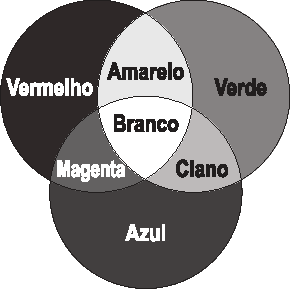
\includegraphics[width=.7\columnwidth]{subareas/ciencias_natureza/fisica-1.pdf}
\end{center}
A protanopia é um tipo de daltonismo em que há diminuição ou ausência de receptores da cor vermelha. Considere um teste com dois voluntários: uma pessoa com visão normal e outra com caso severo de protanopia. Nesse teste, eles devem escrever a cor dos cartões que lhes são mostrados. São utilizadas as cores indicadas na figura.\\
Para qual cartão os dois voluntários identificarão a mesma cor?
\begin{alternativas}
\item Vermelho
\item Magenta
\item Amarelo
\item Branco
\item Azul
\end{alternativas}

\questao
\textit{Slackline} é um esporte no qual o atleta deve se equilibrar e executar manobras estando sobre uma fita esticada. Para a prática do esporte, as duas extremidades da fita são fixadas de forma que ela fique a alguns centímetros do solo. Quando uma atleta de massa igual a 80 kg está exatamente no meio da fita, essa se desloca verticalmente, formando um ângulo de 10° com a horizontal, como esquematizado na figura. Sabe-se que a aceleração da gravidade é igual a 10 $m/s^2$, $\cos (10^\circ) = 0,98$ e $\sen (10^{\circ}) = 0,17$.
\begin{center}
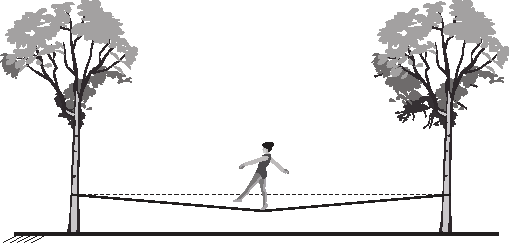
\includegraphics[width=\columnwidth]{subareas/ciencias_natureza/fisica-2.pdf}
\end{center}
Qual é a força que a fita exerce em cada uma das árvores por causa da presença da atleta?
\begin{alternativas}
\item $4,0 \times 102$ N
\item $4,1 \times 102$ N
\item $8,0 \times 102$ N
\item $2,4 \times 103$ N
\item $4,7 \times 103$ N
\end{alternativas}

\questao
Uma casa tem um cabo elétrico mal dimensionado, de resistência igual a 10 $\Omega$, que a conecta à rede elétrica de 120 V. Nessa casa, cinco lâmpadas, de resistência igual a 200 $\Omega$, estão conectadas ao mesmo circuito que uma televisão de resistência igual a 50 $\Omega$, conforme ilustrado no esquema. A televisão funciona apenas com tensão entre 90 V e 130 V.
\begin{center}
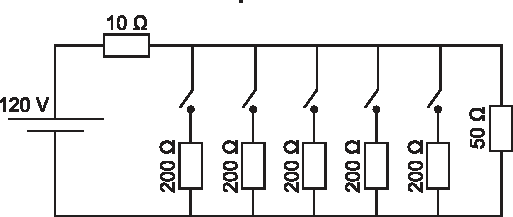
\includegraphics[width=\columnwidth]{subareas/ciencias_natureza/fisica-3.pdf}
\end{center}
O número máximo de lâmpadas que podem ser ligadas sem que a televisão pare de funcionar é:
\begin{alternativas}
\item 1
\item 2
\item 3
\item 4
\item 5
\end{alternativas}

\questao
\citacao{
Em 1808, Dalton publicou o seu famoso livro intitulado Um novo sistema de filosofia química (do original A New System of Chemical Philosophy), no qual continha os cinco postulados que serviam como alicerce da primeira teoria atômica da matéria fundamentada no método científico. Esses postulados são numerados a seguir:\\
1. A matéria é constituída de átomos indivisíveis.\\
2. Todos os átomos de um dado elemento químico são idênticos em massa e em todas as outras propriedades. \\
3. Diferentes elementos químicos têm diferentes tipos de átomos; em particular, seus átomos têm diferentes massas.\\
4. Os átomos são indestrutíveis e nas reações químicas mantêm suas identidades.\\
5. Átomos de elementos combinam com átomos de outros elementos em proporções de números inteiros pequenos para formar compostos.\\
Após o modelo de Dalton, outros modelos baseados em outros dados experimentais evidenciaram, entre outras coisas, a natureza elétrica da matéria, a composição e organização do átomo e a quantização da energia no modelo atômico.}{
OXTOBY, D. W.; GILLIS, H. P.; BUTLER, L. J. Principles of Modern Chemistry. Boston: Cengage Learning, 2012 (adaptado).}
Com base no modelo atual que descreve o átomo, qual dos postulados de Dalton ainda é considerado correto?
\begin{alternativas}
\item 1
\item 2
\item 3
\item 4
\item 5
\end{alternativas}

\questao
\citacao{
Quando se considera a extrema velocidade com que a luz se espalha por todos os lados e que, quando vêm de diferentes lugares, mesmo totalmente opostos, [os raios luminosos] se atravessam uns aos outros sem se atrapalharem, compreende-se que, quando vemos um objeto luminoso, isso não poderia ocorrer pelo transporte de uma matéria que venha do objeto até nós, como uma flecha ou bala atravessa o ar; pois certamente isso repugna bastante a essas duas propriedades da luz, principalmente a última.}{
HUYGENS, C. In: MARTINS, R. A. Tratado sobre a luz, de Cristian Huygens. Caderno de História e Filosofia da Ciência, supl. 4, 1986.}
O texto contesta que concepção acerca do comportamento da luz?
\begin{alternativas}
\item O entendimento de que a luz precisa de um meio de propagação, difundido pelos defensores da existência do éter.
\item O modelo ondulatório para a luz, o qual considera a possibilidade de interferência entre feixes luminosos.
\item O modelo corpuscular defendido por Newton, que descreve a luz como um feixe de partículas.
\item A crença na velocidade infinita da luz, defendida pela maioria dos filósofos gregos.
\item A ideia defendida pelos gregos de que a luz era produzida pelos olhos.
\end{alternativas}

\questao
\citacao{
A gripe é uma infecção respiratória aguda de curta duração causada pelo vírus influenza. Ao entrar no nosso organismo pelo nariz, esse vírus multiplica-se, disseminando-se para a garganta e demais partes das vias respiratórias, incluindo os pulmões.
O vírus influenza é uma partícula esférica que tem um diâmetro interno de 0,00011 mm.
}{
Disponível em: www.gripenet.pt. Acesso em: 2 nov. 2013 (adaptado).}
Em notação científica, o diâmetro interno do vírus influenza, em mm, é:
\begin{alternativas}
\item $1,1 \times 10^{-1}$
\item $1,1 \times 10^{-2}$
\item $1,1 \times 10^{-3}$
\item $1,1 \times 10^{-4}$
\item $1,1 \times 10^{-5}$
\end{alternativas}

\questao
Os exercícios físicos são recomendados para o bom funcionamento do organismo, pois aceleram o metabolismo e, em consequência, elevam o consumo de calorias. No gráfico, estão registrados os valores calóricos, em kcal, gastos em cinco diferentes atividades físicas, em função do tempo dedicado às atividades, contado em minuto.
\begin{center}
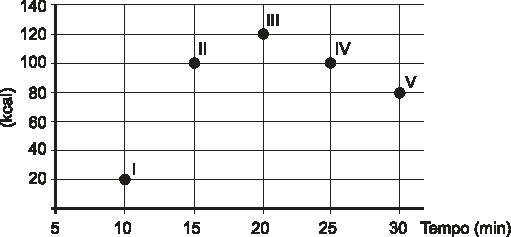
\includegraphics[width=\columnwidth]{subareas/ciencias_natureza/fisica-4.pdf}
\end{center}
Qual dessas atividades físicas proporciona o maior consumo de quilocalorias por minuto?
\begin{alternativas}
\item I
\item II
\item III
\item IV
\item V
\end{alternativas}

\questao
O serviço de meteorologia de uma cidade emite relatórios diários com a previsão do tempo. De posse dessas informações, a prefeitura emite três tipos de alertas para a população:
\begin{itemize}
\item Alerta cinza: deverá ser emitido sempre que a previsão do tempo estimar que a temperatura será inferior a 10 °C, e a umidade relativa do ar for inferior a 40\%;
\item Alerta laranja: deverá ser emitido sempre que a previsão do tempo estimar que a temperatura deve variar entre 35 °C e 40 °C, e a umidade relativa do ar deve ficar abaixo de 30\%;
\item Alerta vermelho: deverá ser emitido sempre que a previsão do tempo estimar que a temperatura será superior a 40 °C, e a umidade relativa do ar for inferior a 25\%.
\end{itemize}
Um resumo da previsão do tempo nessa cidade, para um período de 15 dias, foi apresentado no gráfico.
\begin{center}
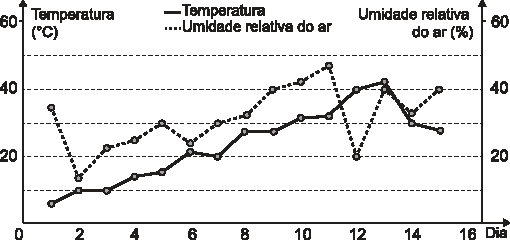
\includegraphics[width=\columnwidth]{subareas/ciencias_natureza/fisica-5.pdf}
\end{center}
Decorridos os 15 dias de validade desse relatório, um funcionário percebeu que, no período a que se refere o gráfico, foram emitidos os seguintes alertas:
\begin{itemize}
\item Dia 1: alerta cinza;
\item Dia 12: alerta laranja;
\item Dia 13: alerta vermelho.
\end{itemize}
Em qual(is) desses dias o(s) aviso(s) foi(ram) emitido(s) corretamente?
\begin{alternativas}
\item 1
\item 12
\item 1 e 12
\item 1 e 13
\item 1, 12 e 13
\end{alternativas}

\questao
Nos seis cômodos de uma casa há sensores de presença posicionados de forma que a luz de cada cômodo acende assim que uma pessoa nele adentra, e apaga assim que a pessoa se retira desse cômodo. Suponha que o acendimento e o desligamento sejam instantâneos.\\
O morador dessa casa visitou alguns desses cômodos, ficando exatamente um minuto em cada um deles. O gráfico descreve o consumo acumulado de energia, em watt $\times$ minuto, em função do tempo t, em minuto, das lâmpadas de LED dessa casa, enquanto a figura apresenta a planta baixa da casa, na qual os cômodos estão numerados de 1 a 6, com as potências das respectivas lâmpadas indicadas.
\begin{center}
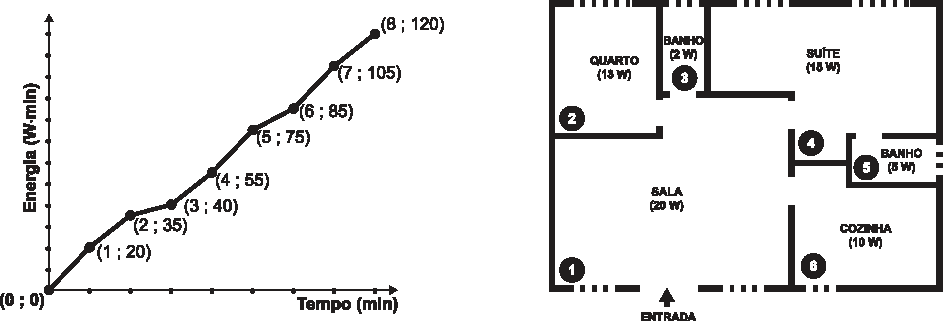
\includegraphics[width=\columnwidth]{subareas/ciencias_natureza/fisica-6.pdf}
\end{center}
A sequência de deslocamentos pelos cômodos, conforme o consumo de energia apresentado no gráfico, é:
\begin{alternativas}
\item $1 \to 4 \to 5 \to 4 \to 1 \to 6 \to 1 \to 4$
\item $1 \to 2 \to 3 \to 1 \to 4 \to 1 \to 4 \to 4$
\item $1 \to 4 \to 5 \to 4 \to 1 \to 6 \to 1 \to 2 \to 3$
\item $1 \to 2 \to 3 \to 5 \to 4 \to 1 \to 6 \to 1 \to 4$
\item $1 \to 4 \to 2 \to 3 \to 5 \to 1 \to 6 \to 1 \to 4$
\end{alternativas}

\questao \label{cn-last}
Muitos smartphones e tablets não precisam mais de teclas, uma vez que todos os comandos podem ser dados ao se pressionar a própria tela. Inicialmente essa tecnologia foi proporcionada por meio das telas resistivas, formadas basicamente por duas camadas de material condutor transparente que não se encostam até que alguém se pressione, modificando a resistência total do circuito de acordo com o ponto onde ocorre o toque. A imagem é uma simplificação do circuito formado pelas placas, em que A e B representam pontos onde o circuito pode ser fechado por meio do toque.
\begin{center}
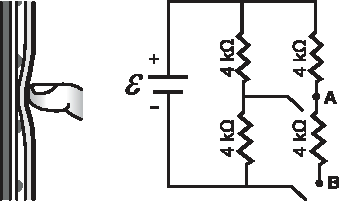
\includegraphics[width=\columnwidth]{subareas/ciencias_natureza/fisica-7.pdf}
\end{center}
Qual é a resistência equivalente no circuito provocada por um toque que fecha o circuito no ponto A?
\begin{alternativas}
\item 1,3 k$\Omega$
\item 4,0 k$\Omega$
\item 6,0 k$\Omega$
\item 6,7 k$\Omega$
\item 12,0 k$\Omega$
\end{alternativas}